%% This file was auto-generated by IPython.
%% Conversion from the original notebook file:
%% Exercise 9.ipynb
%%
\documentclass[11pt,english]{article}

%% This is the automatic preamble used by IPython.  Note that it does *not*
%% include a documentclass declaration. The documentclass is added at runtime
%% to the overall document.
\usepackage{fancyhdr}
\usepackage{amsmath}
\usepackage{amssymb}
\usepackage{graphicx}
\usepackage{ucs}
\usepackage[utf8x]{inputenc}

% needed for markdown enumerations to work
\usepackage{enumerate}

% Slightly bigger margins than the latex defaults
\usepackage{geometry}
\geometry{verbose,tmargin=3cm,bmargin=3cm,lmargin=2.5cm,rmargin=2.5cm}

% Define a few colors for use in code, links and cell shading
\usepackage{color}
\definecolor{orange}{cmyk}{0,0.4,0.8,0.2}
\definecolor{darkorange}{rgb}{.71,0.21,0.01}
\definecolor{darkgreen}{rgb}{.12,.54,.11}
\definecolor{myteal}{rgb}{.26, .44, .56}
\definecolor{gray}{gray}{0.45}
\definecolor{lightgray}{gray}{.95}
\definecolor{mediumgray}{gray}{.8}
\definecolor{inputbackground}{rgb}{.95, .95, .85}
\definecolor{outputbackground}{rgb}{.95, .95, .95}
\definecolor{traceback}{rgb}{1, .95, .95}

% Framed environments for code cells (inputs, outputs, errors, ...).  The
% various uses of \unskip (or not) at the end were fine-tuned by hand, so don't
% randomly change them unless you're sure of the effect it will have.
\usepackage{framed}

% remove extraneous vertical space in boxes
\setlength\fboxsep{0pt}

% codecell is the whole input+output set of blocks that a Code cell can
% generate.

% TODO: unfortunately, it seems that using a framed codecell environment breaks
% the ability of the frames inside of it to be broken across pages.  This
% causes at least the problem of having lots of empty space at the bottom of
% pages as new frames are moved to the next page, and if a single frame is too
% long to fit on a page, it will completely stop latex from compiling the
% document.  So unless we figure out a solution to this, we'll have to instead
% leave the codecell env. as empty.  I'm keeping the original codecell
% definition here (a thin vertical bar) for reference, in case we find a
% solution to the page break issue.

%% \newenvironment{codecell}{%
%%     \def\FrameCommand{\color{mediumgray} \vrule width 1pt \hspace{5pt}}%
%%    \MakeFramed{\vspace{-0.5em}}}
%%  {\unskip\endMakeFramed}

% For now, make this a no-op...
\newenvironment{codecell}{}

 \newenvironment{codeinput}{%
   \def\FrameCommand{\colorbox{inputbackground}}%
   \MakeFramed{\advance\hsize-\width \FrameRestore}}
 {\unskip\endMakeFramed}

\newenvironment{codeoutput}{%
   \def\FrameCommand{\colorbox{outputbackground}}%
   \vspace{-1.4em}
   \MakeFramed{\advance\hsize-\width \FrameRestore}}
 {\unskip\medskip\endMakeFramed}

\newenvironment{traceback}{%
   \def\FrameCommand{\colorbox{traceback}}%
   \MakeFramed{\advance\hsize-\width \FrameRestore}}
 {\endMakeFramed}

% Use and configure listings package for nicely formatted code
\usepackage{listingsutf8}
\lstset{
  language=python,
  inputencoding=utf8x,
  extendedchars=\true,
  aboveskip=\smallskipamount,
  belowskip=\smallskipamount,
  xleftmargin=2mm,
  breaklines=true,
  basicstyle=\small \ttfamily,
  showstringspaces=false,
  keywordstyle=\color{blue}\bfseries,
  commentstyle=\color{myteal},
  stringstyle=\color{darkgreen},
  identifierstyle=\color{darkorange},
  columns=fullflexible,  % tighter character kerning, like verb
}

% The hyperref package gives us a pdf with properly built
% internal navigation ('pdf bookmarks' for the table of contents,
% internal cross-reference links, web links for URLs, etc.)
\usepackage{hyperref}
\hypersetup{
  breaklinks=true,  % so long urls are correctly broken across lines
  colorlinks=true,
  urlcolor=blue,
  linkcolor=darkorange,
  citecolor=darkgreen,
  }

% hardcode size of all verbatim environments to be a bit smaller
\makeatletter
\g@addto@macro\@verbatim\small\topsep=0.5em\partopsep=0pt
\makeatother

% Prevent overflowing lines due to urls and other hard-to-break entities.
\sloppy

\newcommand{\HRule}{\rule{\linewidth}{0.5mm}}
\title{\bf K-means Clustering}
\author{Xugang Zhou \\ Fangzhou Yang}
\pagestyle{fancy}
\lhead{{\bf Machine Intelligence 2 SS2013}}
\rhead{Exercise 09}
\renewcommand{\headrulewidth}{0.4pt}

\begin{document}
\begin{titlepage}
\begin{center}
\vfill
\textsc{\LARGE Machine Intelligence 2}\\[1.5cm]
\textsc{\Large Exercise 09}\\[0.5cm]

\HRule \\[0.4cm]
{\huge \bfseries K-means Clustering}\\[0.4cm]
\HRule \\[1.5cm]
\begin{minipage}{0.4\textwidth}
\begin{flushleft} \large
\emph{Group Members:}\\
Xugang \textsc{Zhou}\\
Fangzhou \textsc{Yang}
\end{flushleft}
\end{minipage}
\begin{minipage}{0.4\textwidth}
\begin{flushright} \large
\emph{Tutor:} \\
Timm \textsc{Lochmann} \\
\end{flushright}
\end{minipage}
\vfill
{\large \today}\\
\end{center}
\end{titlepage}
\thispagestyle{fancy}

\section{9.1 K-Means Clustering}

\begin{codecell}
\begin{codeinput}
\begin{lstlisting}
#function
from numpy import *
import matplotlib
import matplotlib.pyplot as plt

def plotScatter(X,Y,title,c,ran):
    fig = plt.figure()
    ax = fig.add_subplot(111)
    ax.axis([-ran,ran,-ran,ran])
    ax.plot(X,Y,c+'.')
    ax.set_title(title)
    plt.show()

def plotCluster(X,Y,title,colors,ran,assign, W):
    fig = plt.figure()
    ax = fig.add_subplot(111)
    ax.axis([-ran,ran,-ran,ran])
    for i in range (len(X)):
        p = assign[i]
        ax.plot(X[i],Y[i],colors[p]+'.')
    for i in range (len(W)):
        ax.plot(W[i][0],W[i][1],colors[i]+'D')
        ax.plot(W[i][0],W[i][1],'y'+'H')
    ax.set_title(title)
    plt.show()
    
def plotLine(data,title):
    fig = plt.figure()
    ax = fig.add_subplot(111)
    xaxis = [i+1 for i in range(len(data))]
    ax.plot(xaxis,data,'.-')
    ax.set_title(title)
    plt.show()
    
def distance(x1,y1,x2,y2):
    return math.sqrt((y2-y1)**2 + (x2-x1)**2)

def assignPoint(W,x,y):
    k = len(W)
    for i in range(k):
        if(i==0):
            min_distance = distance(W[i][0],W[i][1],x,y)
            min_p = i
        else:
            d = distance(W[i][0],W[i][1],x,y)
            if(d < min_distance):
                min_distance = d
                min_p = i
    return min_p

def drawBoundary(X,Y,title,colors,ran,assign, W, fine):
    fig = plt.figure()
    ax = fig.add_subplot(111)
    ax.axis([-ran,ran,-ran,ran])
    for i in range (len(X)):
        p = assign[i]
        ax.plot(X[i],Y[i],colors[p]+'.')
    for i in range (len(W)):
        ax.plot(W[i][0],W[i][1],colors[i]+'D')
        ax.plot(W[i][0],W[i][1],'y'+'H')
    ax.set_title(title)
    
    ran = float(ran)
    unit = 2*ran/fine
    print 'unit',unit
    for i in range(fine):
        x = -ran + i*unit
        for j in range(fine):
            y = -ran + j*unit
            #print x,y
            p0 = assignPoint(W,x,y)
            p1 = assignPoint(W,x+unit,y)
            p2 = assignPoint(W,x-unit,y)
            p3 = assignPoint(W,x,y+unit)
            p4 = assignPoint(W,x,y-unit)
            if(p0==p1 and p1==p2 and p2==p3 and p3==p4):
                continue
            else:
                ax.plot(x,y,'y.')
    plt.show()
\end{lstlisting}
\end{codeinput}
\end{codecell}
\begin{codecell}
\begin{codeinput}
\begin{lstlisting}
#read data
data = loadtxt("cluster.dat")
print data.shape

X = data[0,:]
Y = data[1,:]

plotScatter(X,Y,"Scatter Plot", 'g', 3)
\end{lstlisting}
\end{codeinput}
\begin{codeoutput}
\begin{verbatim}
(2, 500)
\end{verbatim}
\begin{center}
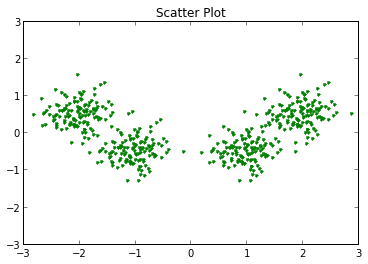
\includegraphics[width=0.7\textwidth]{Exercise_9_files/Exercise_9_fig_00.png}
\par
\end{center}
\end{codeoutput}
\end{codecell}
\begin{codecell}
\begin{codeinput}
\begin{lstlisting}
def distance(x1,y1,x2,y2):
    return math.sqrt((y2-y1)**2 + (x2-x1)**2)

def K_Means(X,Y,k,t_max,W_init):
    assign = [0 for i in range(len(X))]
    error = [0 for i in range(t_max)]
    W = W_init[:][:]
    for i in range (t_max):
        for n in range (len(X)):
            for p in range(k):
                if(p == 0):
                    min_distance = distance(X[n],Y[n],W[p][0],W[p][1])
                    min_p = p
                else:
                    tmp = distance(X[n],Y[n],W[p][0],W[p][1])
                    if (tmp < min_distance):
                        min_distance = tmp
                        min_p = p
            assign[n] = min_p
        
        #draw
        print 'iteration ' + str(i+1) +' done!'
        colors = ['r','g','b','c','m']
        plotCluster(X,Y,"Clustering(k="+str(k)+")", colors, 3, assign, W)
        
        #update W
        count = [0 for o in range(k)]
        for p in range(k):
            W[p][0] = 0
            W[p][1] = 0
        for n in range(len(X)):
            tmp = assign[n]
            W[tmp][0] += X[n]
            W[tmp][1] += Y[n]
            count[tmp] += 1
        for p in range(k):
            if(count[p] >0):
                W[p][0] /= count[p]
                W[p][1] /= count[p]
        
        #claculate the error
        error[i] = 0 
        for n in range(len(X)):
            error[i] += distance(X[n],Y[n],W[assign[n]][0],W[assign[n]][1])
        error[i] /= 2*len(X)                                                     
    return assign,error,W
\end{lstlisting}
\end{codeinput}
\end{codecell}
\begin{codecell}
\begin{codeinput}
\begin{lstlisting}
#init W
def init_w(k):
    random.seed(100)
    W_init = [[0 for j in range(2)] for i in range(k)]
    for p in range(k):
        W_init[p][0] = random.random() * 6 - 3
        W_init[p][1] = random.random() * 6 -3
    return W_init
\end{lstlisting}
\end{codeinput}
\end{codecell}
\begin{codecell}
\begin{codeinput}
\begin{lstlisting}
# k=2
t_max = 5

k = 2
W_init = init_w(k)
print matrix(W_init)


assign,error,W = K_Means(X,Y,k,t_max,W_init)



\end{lstlisting}
\end{codeinput}
\begin{codeoutput}
\begin{verbatim}
[[ 0.26042965 -1.32978369]
 [-0.45289446  2.06865679]]
iteration 1 done!
\end{verbatim}
\begin{center}
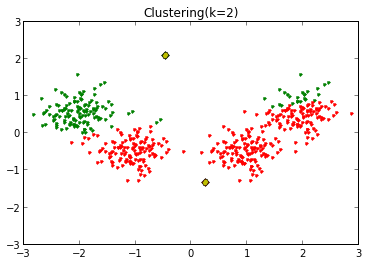
\includegraphics[width=0.7\textwidth]{Exercise_9_files/Exercise_9_fig_01.png}
\par
\end{center}
\begin{verbatim}
iteration 2 done!
\end{verbatim}
\begin{center}
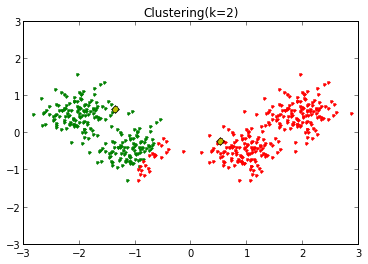
\includegraphics[width=0.7\textwidth]{Exercise_9_files/Exercise_9_fig_02.png}
\par
\end{center}
\begin{verbatim}
iteration 3 done!
\end{verbatim}
\begin{center}
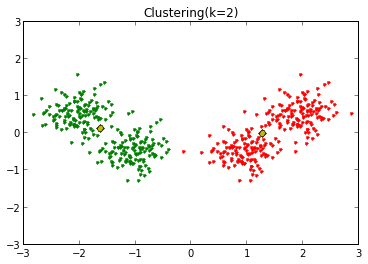
\includegraphics[width=0.7\textwidth]{Exercise_9_files/Exercise_9_fig_03.png}
\par
\end{center}
\begin{verbatim}
iteration 4 done!
\end{verbatim}
\begin{center}
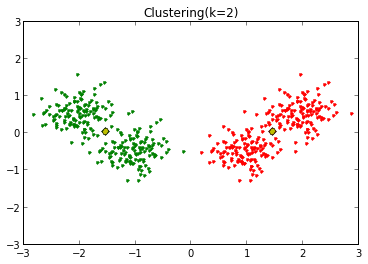
\includegraphics[width=0.7\textwidth]{Exercise_9_files/Exercise_9_fig_04.png}
\par
\end{center}
\begin{verbatim}
iteration 5 done!
\end{verbatim}
\begin{center}
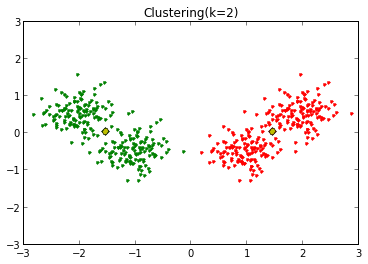
\includegraphics[width=0.7\textwidth]{Exercise_9_files/Exercise_9_fig_05.png}
\par
\end{center}
\end{codeoutput}
\end{codecell}
\begin{codecell}
\begin{codeinput}
\begin{lstlisting}
plotLine(error,"Error-Iteration")
\end{lstlisting}
\end{codeinput}
\begin{codeoutput}
\begin{center}
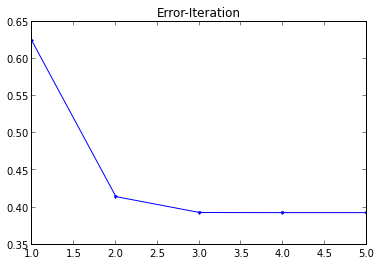
\includegraphics[width=0.7\textwidth]{Exercise_9_files/Exercise_9_fig_06.png}
\par
\end{center}
\end{codeoutput}
\end{codecell}
\begin{codecell}
\begin{codeinput}
\begin{lstlisting}
colors = ['r','g','b','c','m']
drawBoundary(X,Y,"Clustering(k="+str(k)+")",colors, 3, assign, W, 100)
\end{lstlisting}
\end{codeinput}
\begin{codeoutput}
\begin{verbatim}
unit 0.06
\end{verbatim}
\begin{center}
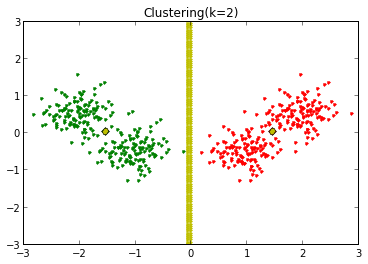
\includegraphics[width=0.7\textwidth]{Exercise_9_files/Exercise_9_fig_07.png}
\par
\end{center}
\end{codeoutput}
\end{codecell}
\begin{codecell}
\begin{codeinput}
\begin{lstlisting}
# k=3
t_max = 5

k = 3
W_init = init_w(k)
print matrix(W_init)


assign,error,W = K_Means(X,Y,k,t_max,W_init)

\end{lstlisting}
\end{codeinput}
\begin{codeoutput}
\begin{verbatim}
[[ 0.26042965 -1.32978369]
 [-0.45289446  2.06865679]
 [-2.97168686 -2.27058528]]
iteration 1 done!
\end{verbatim}
\begin{center}
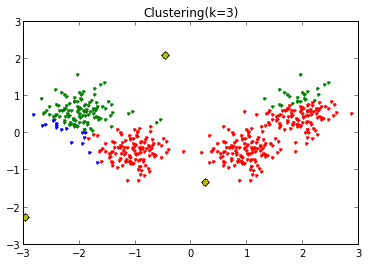
\includegraphics[width=0.7\textwidth]{Exercise_9_files/Exercise_9_fig_08.png}
\par
\end{center}
\begin{verbatim}
iteration 2 done!
\end{verbatim}
\begin{center}
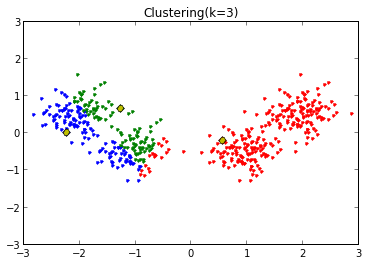
\includegraphics[width=0.7\textwidth]{Exercise_9_files/Exercise_9_fig_09.png}
\par
\end{center}
\begin{verbatim}
iteration 3 done!
\end{verbatim}
\begin{center}
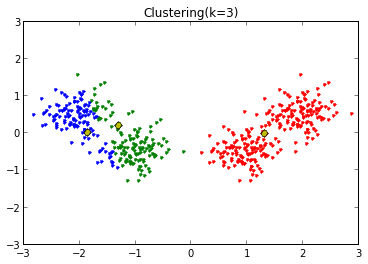
\includegraphics[width=0.7\textwidth]{Exercise_9_files/Exercise_9_fig_10.png}
\par
\end{center}
\begin{verbatim}
iteration 4 done!
\end{verbatim}
\begin{center}
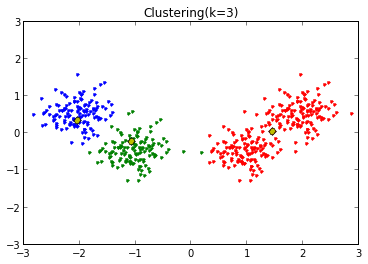
\includegraphics[width=0.7\textwidth]{Exercise_9_files/Exercise_9_fig_11.png}
\par
\end{center}
\begin{verbatim}
iteration 5 done!
\end{verbatim}
\begin{center}
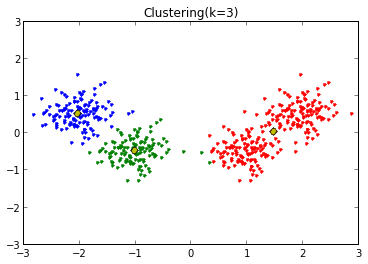
\includegraphics[width=0.7\textwidth]{Exercise_9_files/Exercise_9_fig_12.png}
\par
\end{center}
\end{codeoutput}
\end{codecell}
\begin{codecell}
\begin{codeinput}
\begin{lstlisting}
plotLine(error,"Error-Iteration")
\end{lstlisting}
\end{codeinput}
\begin{codeoutput}
\begin{center}
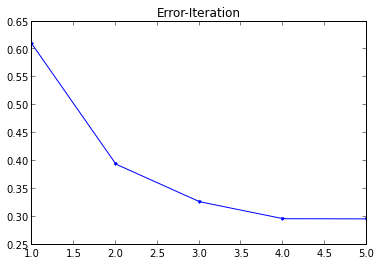
\includegraphics[width=0.7\textwidth]{Exercise_9_files/Exercise_9_fig_13.png}
\par
\end{center}
\end{codeoutput}
\end{codecell}
\begin{codecell}
\begin{codeinput}
\begin{lstlisting}
colors = ['r','g','b','c','m']
drawBoundary(X,Y,"Clustering(k="+str(k)+")",colors, 3, assign, W, 100)
\end{lstlisting}
\end{codeinput}
\begin{codeoutput}
\begin{verbatim}
unit 0.06
\end{verbatim}
\begin{center}
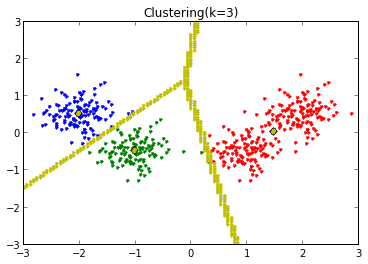
\includegraphics[width=0.7\textwidth]{Exercise_9_files/Exercise_9_fig_14.png}
\par
\end{center}
\end{codeoutput}
\end{codecell}
\begin{codecell}
\begin{codeinput}
\begin{lstlisting}
# k=4
t_max = 5

k = 4
W_init = init_w(k)
print matrix(W_init)


assign,error,W = K_Means(X,Y,k,t_max,W_init)

\end{lstlisting}
\end{codeinput}
\begin{codeoutput}
\begin{verbatim}
[[ 0.26042965 -1.32978369]
 [-0.45289446  2.06865679]
 [-2.97168686 -2.27058528]
 [ 1.02449451  1.95511653]]
iteration 1 done!
\end{verbatim}
\begin{center}
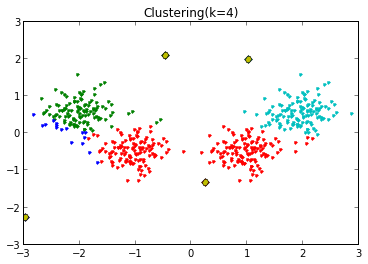
\includegraphics[width=0.7\textwidth]{Exercise_9_files/Exercise_9_fig_15.png}
\par
\end{center}
\begin{verbatim}
iteration 2 done!
\end{verbatim}
\begin{center}
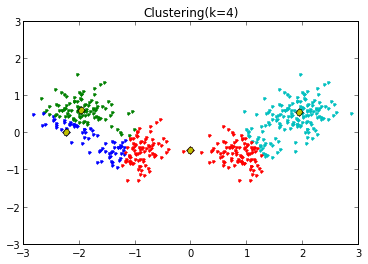
\includegraphics[width=0.7\textwidth]{Exercise_9_files/Exercise_9_fig_16.png}
\par
\end{center}
\begin{verbatim}
iteration 3 done!
\end{verbatim}
\begin{center}
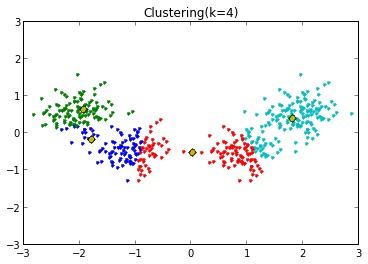
\includegraphics[width=0.7\textwidth]{Exercise_9_files/Exercise_9_fig_17.png}
\par
\end{center}
\begin{verbatim}
iteration 4 done!
\end{verbatim}
\begin{center}
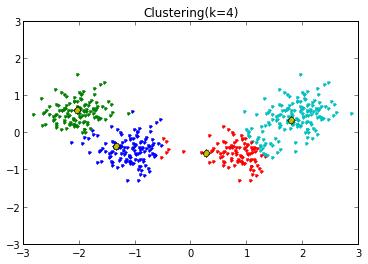
\includegraphics[width=0.7\textwidth]{Exercise_9_files/Exercise_9_fig_18.png}
\par
\end{center}
\begin{verbatim}
iteration 5 done!
\end{verbatim}
\begin{center}
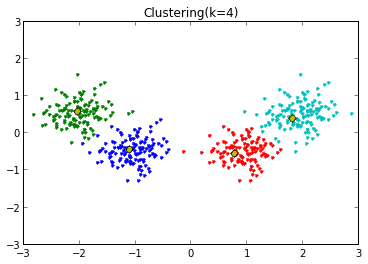
\includegraphics[width=0.7\textwidth]{Exercise_9_files/Exercise_9_fig_19.png}
\par
\end{center}
\end{codeoutput}
\end{codecell}
\begin{codecell}
\begin{codeinput}
\begin{lstlisting}
plotLine(error,"Error-Iteration")
\end{lstlisting}
\end{codeinput}
\begin{codeoutput}
\begin{center}
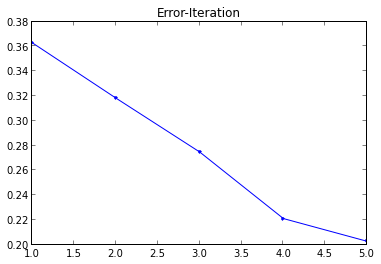
\includegraphics[width=0.7\textwidth]{Exercise_9_files/Exercise_9_fig_20.png}
\par
\end{center}
\end{codeoutput}
\end{codecell}
\begin{codecell}
\begin{codeinput}
\begin{lstlisting}
colors = ['r','g','b','c','m']
drawBoundary(X,Y,"Clustering(k="+str(k)+")",colors, 3, assign, W, 100)
\end{lstlisting}
\end{codeinput}
\begin{codeoutput}
\begin{verbatim}
unit 0.06
\end{verbatim}
\begin{center}
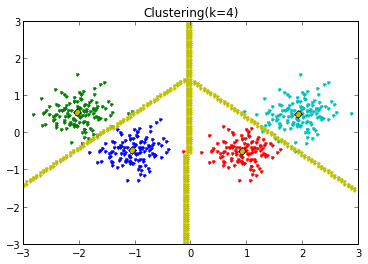
\includegraphics[width=0.7\textwidth]{Exercise_9_files/Exercise_9_fig_21.png}
\par
\end{center}
\end{codeoutput}
\end{codecell}
\begin{codecell}
\begin{codeinput}
\begin{lstlisting}
# k=5
t_max = 5

k = 5
W_init = init_w(k)
print matrix(W_init)


assign,error,W = K_Means(X,Y,k,t_max,W_init)

\end{lstlisting}
\end{codeinput}
\begin{codeoutput}
\begin{verbatim}
[[ 0.26042965 -1.32978369]
 [-0.45289446  2.06865679]
 [-2.97168686 -2.27058528]
 [ 1.02449451  1.95511653]
 [-2.17976046  0.45055998]]
iteration 1 done!
\end{verbatim}
\begin{center}
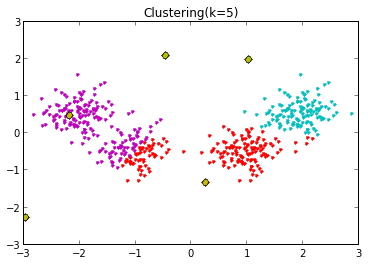
\includegraphics[width=0.7\textwidth]{Exercise_9_files/Exercise_9_fig_22.png}
\par
\end{center}
\begin{verbatim}
iteration 2 done!
\end{verbatim}
\begin{center}
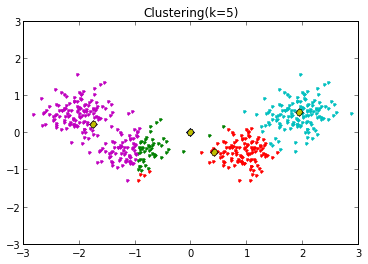
\includegraphics[width=0.7\textwidth]{Exercise_9_files/Exercise_9_fig_23.png}
\par
\end{center}
\begin{verbatim}
iteration 3 done!
\end{verbatim}
\begin{center}
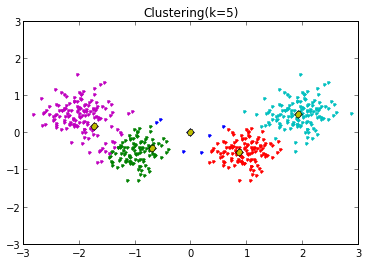
\includegraphics[width=0.7\textwidth]{Exercise_9_files/Exercise_9_fig_24.png}
\par
\end{center}
\begin{verbatim}
iteration 4 done!
\end{verbatim}
\begin{center}
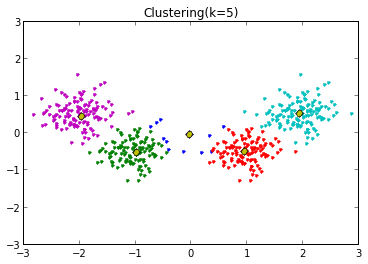
\includegraphics[width=0.7\textwidth]{Exercise_9_files/Exercise_9_fig_25.png}
\par
\end{center}
\begin{verbatim}
iteration 5 done!
\end{verbatim}
\begin{center}
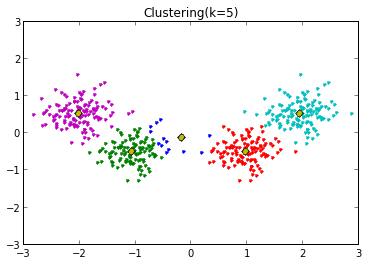
\includegraphics[width=0.7\textwidth]{Exercise_9_files/Exercise_9_fig_26.png}
\par
\end{center}
\end{codeoutput}
\end{codecell}
\begin{codecell}
\begin{codeinput}
\begin{lstlisting}
plotLine(error,"Error-Iteration")
\end{lstlisting}
\end{codeinput}
\begin{codeoutput}
\begin{center}
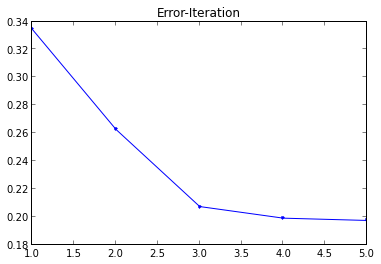
\includegraphics[width=0.7\textwidth]{Exercise_9_files/Exercise_9_fig_27.png}
\par
\end{center}
\end{codeoutput}
\end{codecell}
\begin{codecell}
\begin{codeinput}
\begin{lstlisting}
colors = ['r','g','b','c','m']
drawBoundary(X,Y,"Clustering(k="+str(k)+")",colors, 3, assign, W, 100)
\end{lstlisting}
\end{codeinput}
\begin{codeoutput}
\begin{verbatim}
unit 0.06
\end{verbatim}
\begin{center}
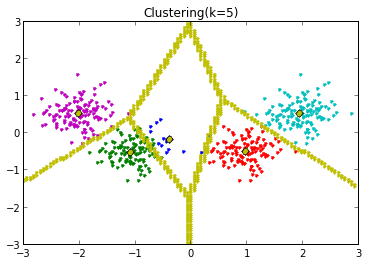
\includegraphics[width=0.7\textwidth]{Exercise_9_files/Exercise_9_fig_28.png}
\par
\end{center}
\end{codeoutput}
\end{codecell}
\section{9.2 Online K-Means Clustering}

\begin{codecell}
\begin{codeinput}
\begin{lstlisting}
#intiliazation
#init W
def init_w_online(k):
    random.seed(100)
    W_init = [[0 for j in range(2)] for i in range(k)]
    for p in range(k):
        W_init[p][0] = random.random() * 4 - 2
        W_init[p][1] = random.random() * 4 -2
    return W_init

t_max = 2* len(X)
k = 4
W_init = init_w_online(k)
print 'W_init'
print matrix(W_init)
eta0 = 0.05
eta = eta0
print 'eta_init:' , eta0
tao = 0.99
print 'tao_init:', tao
\end{lstlisting}
\end{codeinput}
\begin{codeoutput}
\begin{verbatim}
W_init
[[ 0.17361977 -0.88652246]
 [-0.30192964  1.37910453]
 [-1.98112458 -1.51372352]
 [ 0.68299634  1.30341102]]
eta_init: 0.05
tao_init: 0.99
\end{verbatim}
\end{codeoutput}
\end{codecell}
\begin{codecell}
\begin{codeinput}
\begin{lstlisting}
#online K_Means
def K_Means_online(X,Y,k,t_max,W_init):
    assign = [0 for i in range(len(X))]
    W = W_init[:][:]
    delta_w = [0,0]
    error = [0 for i in range(t_max)]
    for t in range(t_max):
        n = t%len(X)
        if(t<t_max/4):
            eta = eta0
        else:
            eta = tao * eta
        p = assignPoint(W,X[n],Y[n])
        assign[n] = p
        delta_w[0] = eta*(X[n] - W[p][0])
        delta_w[1] = eta*(Y[n] - W[p][1])
        W[p][0] += delta_w[0]
        W[p][1] += delta_w[1]
        
        #plot
        #print 'iteration ' + str(t+1) +' done!'
        if(t==0 or t==int(float(t_max)/3) or t==int(float(t_max)/3*2) or t==t_max-1):
        #if(:1)
            colors = ['r','g','b','c','m']
            print 'iteration ' + str(t+1) +' done!'
            plotCluster(X,Y,"Clustering(k="+str(k)+")", colors, 3, assign, W)   
   
        #claculate the error
        error[t]=0
        for j in range(len(X)):
            error[t] += distance(X[j],Y[j],W[assign[j]][0],W[assign[j]][1])
        error[t] /= 2*len(X)  
        
    return assign,W,error
\end{lstlisting}
\end{codeinput}
\end{codecell}
\begin{codecell}
\begin{codeinput}
\begin{lstlisting}
assign,W,error = K_Means_online(X,Y,k,t_max,W_init)
\end{lstlisting}
\end{codeinput}
\begin{codeoutput}
\begin{verbatim}
iteration 1 done!
\end{verbatim}
\begin{center}
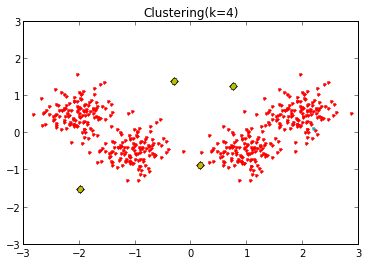
\includegraphics[width=0.7\textwidth]{Exercise_9_files/Exercise_9_fig_29.png}
\par
\end{center}
\begin{verbatim}
iteration 334 done!
\end{verbatim}
\begin{center}
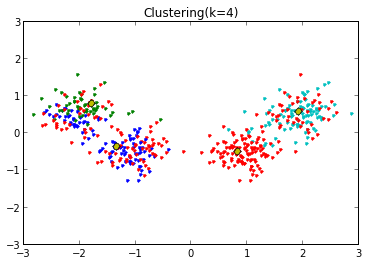
\includegraphics[width=0.7\textwidth]{Exercise_9_files/Exercise_9_fig_30.png}
\par
\end{center}
\begin{verbatim}
iteration 667 done!
\end{verbatim}
\begin{center}
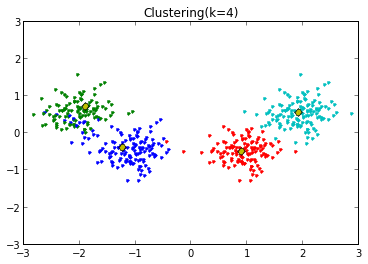
\includegraphics[width=0.7\textwidth]{Exercise_9_files/Exercise_9_fig_31.png}
\par
\end{center}
\begin{verbatim}
iteration 1000 done!
\end{verbatim}
\begin{center}
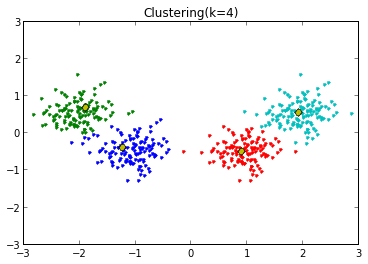
\includegraphics[width=0.7\textwidth]{Exercise_9_files/Exercise_9_fig_32.png}
\par
\end{center}
\end{codeoutput}
\end{codecell}
\begin{codecell}
\begin{codeinput}
\begin{lstlisting}
plotLine(error,"Error-Iteration")
\end{lstlisting}
\end{codeinput}
\begin{codeoutput}
\begin{center}
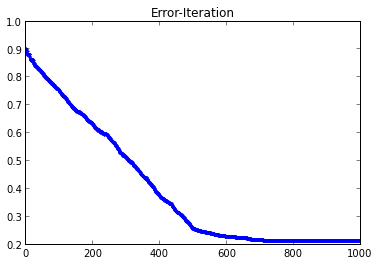
\includegraphics[width=0.7\textwidth]{Exercise_9_files/Exercise_9_fig_33.png}
\par
\end{center}
\end{codeoutput}
\end{codecell}
\begin{codecell}
\begin{codeinput}
\begin{lstlisting}
colors = ['r','g','b','c','m']
drawBoundary(X,Y,"Clustering(k="+str(k)+")",colors, 3, assign, W, 100)
\end{lstlisting}
\end{codeinput}
\begin{codeoutput}
\begin{verbatim}
unit 0.06
\end{verbatim}
\begin{center}
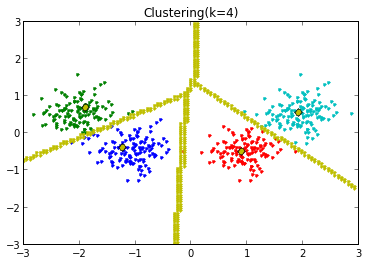
\includegraphics[width=0.7\textwidth]{Exercise_9_files/Exercise_9_fig_34.png}
\par
\end{center}
\end{codeoutput}
\end{codecell}

\end{document}
